% TeX Live 2025's cleveref first aid records appendix sections as sections
% unless the section counter is explicitly aliased after \appendix.
\crefalias{section}{appendix}
\section{Proofs}\label{sec:appendix-acpc-proofs}

\paragraph{Proof of \Cref{prop:target-free-error-drift}.}
Let $u=\bar G_{\mathbf a}(E_\theta(h))$,
$v=\bar G_{\mathbf a}(E_\theta(\tilde h))$, and $y=Y_{\mathbf a}^H$. Both
errors use the same target $y$ in the weighted rollout space of
\Cref{eq:acpc-h}. The reverse triangle inequality gives
\begin{align}
|e_{\tilde h}-e_h|
&=\bigl|\,\|v-y\|_2-\|u-y\|_2\,\bigr| \\
&\le \|(v-y)-(u-y)\|_2
=\|v-u\|_2
=\mathrm{ACPC}_H(h,\tilde h,\mathbf a).
\end{align}
The one-sided error increase satisfies the same bound because
$(e_{\tilde h}-e_h)_+\le|e_{\tilde h}-e_h|$.

\paragraph{Proof of \Cref{prop:exact-cost-certificate}.}
For a single candidate, omit the index. Let $r=\|\tilde x-x\|_2$ and
$A=\mathrm{ACPC}_H(h,\tilde h,\mathbf a)$. Since $r$ is the final-step
displacement in ACPC, its definition gives
\[
\alpha_H r^2\leq A^2.
\]
Thus, $r\leq A/\sqrt{\alpha_H}$. The difference between the two squared costs
factors as
\begin{align}
|\tilde C-C|
&=\bigl|\|\tilde x-g\|_2^2-\|x-g\|_2^2\bigr| \\
&=\bigl|\langle \tilde x-x,\tilde x+x-2g\rangle\bigr| \\
&\le \|\tilde x-x\|_2\,\|\tilde x+x-2g\|_2 \\
&\le r\bigl(2\|x-g\|_2+r\bigr) \\
&\le 2\sqrt C\,\frac{A}{\sqrt{\alpha_H}}
+\frac{A^2}{\alpha_H}.
\end{align}
The first inequality follows from Cauchy--Schwarz, and the second follows from
the triangle inequality. The last inequality uses $r\leq A/\sqrt{\alpha_H}$
and $\|x-g\|_2=\sqrt C$.

\paragraph{Tightness of the prediction-error bound.}
For the prediction-error bound, let
$u$ be a unit vector, set the common target to $Y=0$, and let the two predicted
rollouts be $su$ and $tu$, where $s,t\geq0$. Then
\[
\bigl|\,\|tu\|_2-\|su\|_2\,\bigr|
=\|tu-su\|_2,
\]
so \Cref{eq:target-free-error-drift} holds with equality.

\section{Local-Geometry Case-Study Definitions}
\label{sec:appendix-local-geometry}

This supplementary case study visualizes how augmentation contracts perturbed
views relative to nearby clean histories. We use 128 logged PushT histories.
For each history, we generate one clean view and 18 perturbed views, with six
draws at each standard deviation in $\{0.01,0.04,0.08\}$. Each of the four
qualitative t-SNE panels uses a separate deterministic
projection~\citep{vandermaaten2008tsne}, so
coordinates are not compared across panels.

\begin{figure}[H]
\centering
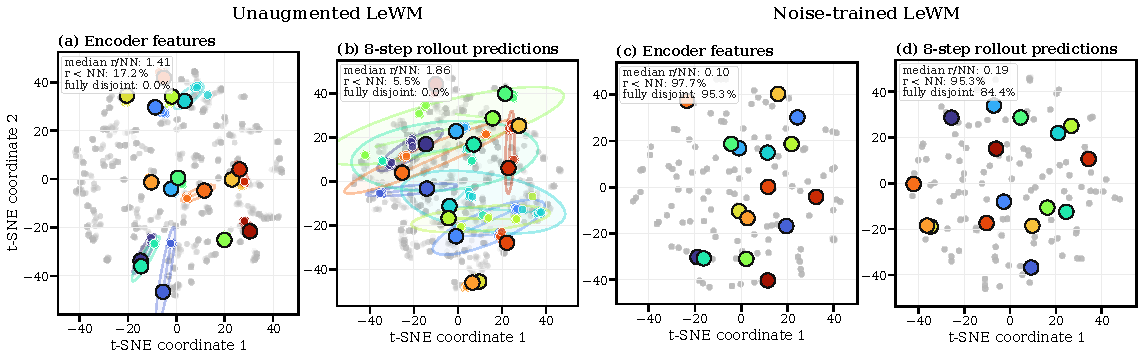
\includegraphics[width=\linewidth]{fig_local_geometry_highd_audit.pdf}
\caption{Local geometry for matched unaugmented (left) and
$\stdmax{}=0.08$ PushT checkpoints (right), at the encoder and after eight
rollout steps. Markers show clean histories and perturbed views; summaries are
computed in the original 192-dimensional space, not in t-SNE.}
\label{fig:local-geometry-highd}
\end{figure}

Without augmentation, median $r/\mathrm{NN}$ is $1.41$ at the encoder and
$1.86$ after rollout, with no fully disjoint perturbation clouds. With
augmentation, the ratios fall to $0.10$ and $0.19$, and the disjoint fractions
rise to $95.3\%$ and $84.4\%$. This is descriptive geometry, not evidence of
task-semantic separation or planning robustness.

We evaluate two representation spaces: the encoder output, denoted by
$\mathcal V=\mathrm{enc}$, and the representation after eight autoregressive
rollout steps, denoted by $\mathcal V=\mathrm{roll}$. The rollout horizon is
$H=8$ (\Cref{sec:acpc-def}). For history $i$, let
$v_{i,\mathcal V}^{(0)}$ be its clean representation and let
$v_{i,\mathcal V}^{(m)}$, $m=1,\ldots,M$ with $M=18$, be its perturbed
representations. In the rollout space, the clean and perturbed views of the
same history use the same recorded action sequence. We then define the sampled
visual radius, the distance to the nearest other clean history, and their ratio:
\begin{align}
r_{i,\mathcal V}^{\mathrm{vis}}
&=\max_{1\leq m\leq M}
\left\|v_{i,\mathcal V}^{(m)}-v_{i,\mathcal V}^{(0)}\right\|_2,
\nonumber\\
d_{i,\mathcal V}^{\mathrm{NN}}
&=\min_{j\neq i}
\left\|v_{i,\mathcal V}^{(0)}-v_{j,\mathcal V}^{(0)}\right\|_2,
\qquad
\rho_{i,\mathcal V}^{\mathrm{local}}
=\frac{r_{i,\mathcal V}^{\mathrm{vis}}}
{d_{i,\mathcal V}^{\mathrm{NN}}}.
\label{eq:local-radius-spacing}
\end{align}
The figures abbreviate $\rho_{i,\mathcal V}^{\mathrm{local}}$ as
$r/\mathrm{NN}$. A value below one means that every sampled perturbation moves
the representation by less than the distance from its clean anchor to any
other clean anchor. A value of at least one means that at least one
perturbation displacement is as large as the nearest-clean distance. This
comparison uses only distance magnitudes: it does not show that a perturbed
representation approaches or overlaps another history, and the nearest clean
history need not differ across a task-relevant state boundary.

The $r/\mathrm{NN}$ ratio considers only the perturbation radius of anchor
$i$. To account for the perturbation radii of both histories, we also compare
their enclosing balls. The ball around anchor $i$ is \emph{fully disjoint} if
it does not intersect the ball around any other anchor:
\begin{equation}
\left\|v_{i,\mathcal V}^{(0)}-v_{j,\mathcal V}^{(0)}\right\|_2
>
r_{i,\mathcal V}^{\mathrm{vis}}+r_{j,\mathcal V}^{\mathrm{vis}}
\quad\text{for every }j\neq i.
\label{eq:local-cloud-disjoint}
\end{equation}
Across the 128 anchors, we report three summaries: the median
$r/\mathrm{NN}$ ratio, the fraction with
$r_{i,\mathcal V}^{\mathrm{vis}}<d_{i,\mathcal V}^{\mathrm{NN}}$, and the
fraction satisfying the fully disjoint condition in
\Cref{eq:local-cloud-disjoint}. The second summary compares each perturbation
radius with the distance to the nearest other clean anchor. The third also
accounts for the perturbation radius around every other anchor. All three
summaries are computed in the original high-dimensional representation;
overlap between the qualitative t-SNE ellipses is not used.

These summaries are descriptive and depend on the sampled histories and
perturbation draws. They compare the encoder output and the final rollout step
but do not examine intermediate predictions. They also do not bound changes
in prediction error or planning cost; those theoretical links are provided by
pairwise ACPC in \Cref{sec:acpc-def}.

\section{Evaluation and Diagnostic Protocol}\label{sec:appendix-A}

This appendix specifies the fixed evaluation and diagnostic protocol used in
the reported results.

\paragraph{Evaluation grid.}
We evaluate LeWM on PushT, TwoRoom, Reacher, and Cube. Each checkpoint is
evaluated with seeds 42, 43, and 44, using 100 episodes per seed. The primary
evaluation adds Gaussian noise with standard deviation $0.08$ to the history
observations while keeping the goal image clean. For each task, the training
grid contains one unaugmented checkpoint and eight checkpoints trained with
full-sequence Gaussian-noise augmentation at
$\stdmax{}\in\{0.01,0.02,\ldots,0.08\}$.

\paragraph{PLDM protocol.}
PLDM is evaluated on the same four tasks and nine-checkpoint training grid as
LeWM, using the same evaluation seeds and number of logged histories. Its
diagnostics use the same clean--perturbed pairing, eight-step rollout horizon,
and SR definition. In the PLDM plots, raw IR is divided by the value of the
unaugmented PLDM checkpoint from the same task and training run.

\paragraph{PLDM results.}\label{sec:exp-pldm-diagnostics}
To test whether the diagnostics are specific to LeWM, we apply the same ACPC,
IR, and SR definitions to PLDM, which uses a different architecture and
training recipe. The evaluated PLDM sweeps show a similar qualitative pattern:
better control performance is associated with lower IR and higher SR
(\Cref{tab:pldm-all-levels}).

\begin{table}[H]
\centering
\caption{\textbf{PLDM over the complete augmented training grid.} Success and SR cells give the unaugmented three-run mean followed by the range of three-run means over all eight augmented levels $\sigma_{\max}^{\mathrm{train}}\in\{0.01,\ldots,0.08\}$; success also gives the unaugmented across-run population SD. Relative IR lists only the augmented range because its unaugmented value is one by construction. No level is selected. The grid ends at $0.08$ and therefore cannot measure an overaugmentation boundary; \Cref{fig:pldm-sweep-diagnostics} gives per-level curves and across-run ranges.}
\label{tab:pldm-all-levels}
\footnotesize
\setlength{\tabcolsep}{5.0pt}
\begin{tabular}{lccc}
\toprule
Task & \shortstack{Planning success (\%)\\unaug. $\to$ augmented range} & \shortstack{Relative IR\\augmented range} & \shortstack{SR\\unaug. $\to$ augmented range} \\
\midrule
TwoRoom & 67.1$\pm$8.0$\to$[95.7, 97.7] & [0.071, 0.440] & 0.082$\to$[0.967, 1.000] \\
PushT & 10.2$\pm$5.9$\to$[20.9, 70.3] & [0.070, 0.866] & 0.228$\to$[0.439, 1.000] \\
Reacher & 53.0$\pm$29.7$\to$[63.0, 82.2] & [0.166, 0.893] & 0.650$\to$[0.887, 1.000] \\
Cube & 45.9$\pm$1.7$\to$[50.6, 53.9] & [0.043, 0.742] & 0.170$\to$[0.637, 1.000] \\
\bottomrule
\end{tabular}
\end{table}


\begin{figure}[H]
\centering
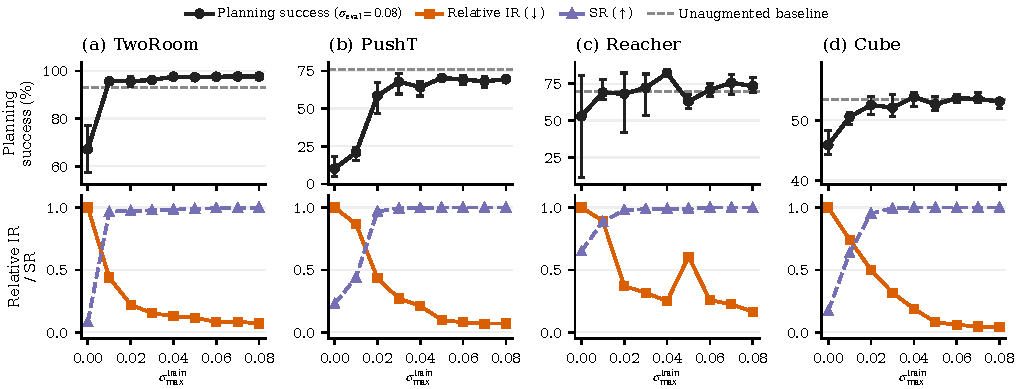
\includegraphics[width=\linewidth]{fig_pldm_sweep_diagnostics.pdf}
\caption{Complete PLDM Gaussian-noise training sweep over three runs. Curves
show three-run means and success bars span the across-run range. The summary in
\Cref{tab:pldm-all-levels} includes every augmented level rather than selecting a recovery
subset.}
\label{fig:pldm-sweep-diagnostics}
\end{figure}

\paragraph{Success-rate criterion.}
For each task and training run, let $S_0$ be the
noisy-observation success rate of the unaugmented checkpoint, and let
$S_{\max}$ be the highest noisy-observation success rate observed in
the fixed nine-checkpoint sweep. A checkpoint meets the success-rate criterion if its
noisy-observation success rate is at least
\[
S_0+0.8(S_{\max}-S_0)
\]
and its clean-observation success rate is no more than five percentage points
below that of the unaugmented checkpoint. At the task level, we call an
augmentation level recovered only when this criterion holds in at least two
of the three training runs. $S_{\max}$ is used only to scale this
recovery label; every level meeting the criterion remains part of the reported
range.

\paragraph{IR protocol.}
We compute IR separately for each task, training run, and checkpoint. To
express rollout divergence relative to the normal motion in each history, we
first compute a clean-motion scale. For anchor $i$, let
$u^{\mathrm{obs}}_{i,0}$ be the projected embedding of the final history
observation, and let $u^{\mathrm{obs}}_{i,1:H}$ be the projected embeddings of
the next $H$ observed clean frames. We define
\begin{equation}
s_i
=Q_{0.50}\!\left(
\left\{\|u^{\mathrm{obs}}_{i,k}-u^{\mathrm{obs}}_{i,k-1}\|_2
\right\}_{k=1}^{H}
\right).
\label{eq:clean-transition-scale}
\end{equation}
Thus, $s_i$ is the median displacement between consecutive clean observations,
including the transition from the final history observation to the first
future observation.

For each anchor, we generate multiple perturbation draws using the visual
shift being evaluated, with five draws for Gaussian noise. For the Gaussian-noise
experiments in \Cref{sec:exp-gaussian-panel}, we use $\sigma=0.08$; the
blur and resize experiments apply their corresponding shifts. For every draw,
we compute eight-step ACPC with uniform weights $\alpha_k=1/H$ and normalize it
by $s_i+\varepsilon_{\mathrm{norm}}$. We average the normalized values across
draws for each anchor and then take the 90th percentile (q90) across anchors.
The result is raw IR in
\Cref{eq:ir-raw}.

SR compares different-state distances with raw IR from the same checkpoint.
For the sweep plots, raw IR is divided by the value of the corresponding
unaugmented checkpoint, as defined in \Cref{eq:ir-relative}. Only the LeWM
cross-task analysis uses relative IR for threshold selection. We use
$\varepsilon_{\mathrm{norm}}=10^{-8}$ in
\Cref{eq:normalized-same-state-radius}.

Across all 108 LeWM checkpoints from the four tasks in the main Gaussian-noise
sweep, zero clean-motion scale occurred only in PushT, at one of the 100
anchors per checkpoint. For this anchor, the denominator reduces to
$\varepsilon_{\mathrm{norm}}$. Excluding it changed relative IR by at most
$0.034$, with only one checkpoint crossing each of the two fixed IR thresholds
examined ($0.1$ and $0.3$). These crossings occurred near the threshold
boundaries. The 90th-percentile aggregation prevents this single extreme value
from directly determining IR.

\Cref{tab:horizon-quantile-sensitivity} reports the results for the tested
rollout horizons and summary quantiles.

\begin{table}[H]
\centering
\caption{Horizon and quantile sensitivity of the IR reduction at fixed evaluation noise $\sigma=0.08$. Each entry is the median, over the three training runs, of the ratio between the IR of the checkpoint trained at the highest augmentation level ($\stdmax{}=0.08$) and that of the unaugmented checkpoint; lower means a larger reduction. q80, q90, and q95 denote the 80th, 90th, and 95th percentiles, respectively. These values are descriptive and do not retune any threshold.}
\label{tab:horizon-quantile-sensitivity}
\small
\setlength{\tabcolsep}{5pt}
\begin{tabular}{lccccccc}
\toprule
& \multicolumn{4}{c}{$q=0.90$ by horizon} & \multicolumn{3}{c}{$H=8$ by quantile} \\
\cmidrule(lr){2-5}\cmidrule(lr){6-8}
Task & H1 & H2 & H4 & H8 & q80 & q90 & q95 \\
\midrule
TwoRoom & 0.05 & 0.04 & 0.05 & 0.06 & 0.06 & 0.06 & 0.06 \\
PushT & 0.06 & 0.07 & 0.06 & 0.09 & 0.07 & 0.09 & 0.09 \\
Reacher & 0.02 & 0.03 & 0.03 & 0.02 & 0.02 & 0.02 & 0.02 \\
Cube & 0.04 & 0.03 & 0.04 & 0.04 & 0.03 & 0.04 & 0.04 \\
\bottomrule
\end{tabular}
\end{table}


\paragraph{SR protocol.}
SR follows \Cref{eq:sr}. We first define a local neighborhood using the
standardized logged endpoint states. Let $d_{0.35}$ be the 35th percentile of
all pairwise distances between different endpoints---that is, the q35 of all off-diagonal Euclidean distances.
This cutoff keeps the comparisons local while retaining an eligible neighbor for most anchors;
\Cref{tab:sr-labels} reports the resulting counts.

For each anchor $i$, we select the nearest history $j(i)$ that has a different
endpoint-state label and lies within distance $d_{0.35}$. If no such history
exists, the anchor is excluded from SR. We roll both histories forward under
the anchor's recorded action sequence $\mathbf a_i$. This sequence was not
generally executed by the neighboring history, but using it for both rollouts
prevents action differences from affecting the comparison. Their normalized
rollout distance is
\begin{equation}
D_i^{\mathrm{diff}}
=
\frac{
\left\|\bar G_{\mathbf a_i}(E_\theta(h_i))
-\bar G_{\mathbf a_i}(E_\theta(h_{j(i)}))\right\|_2
}{s_i+\varepsilon_{\mathrm{norm}}}.
\end{equation}
The pair counts as separated when $D_i^{\mathrm{diff}}$ is greater than raw
q90 IR plus the fixed margin $0.10$.
Prediction errors in the neighbor's rollout under the anchor's actions may
increase the measured separation.

For pairing, the endpoint state is taken after the eight observed future steps
and therefore records the state reached under that trajectory's own actions.
The dataset preprocessor standardizes each state coordinate, and neighborhood
distances use the full standardized state vector. Endpoint-state labels are
constructed by median splits of the task-specific coordinates listed in
\Cref{tab:sr-labels}, using the fixed batch of 100 endpoints generated with
anchor seed 9101. Because the logged endpoints, labels, and neighborhoods are
fixed before checkpoint evaluation, the selected pairs and eligible-anchor
counts are identical across checkpoints and training runs.

\begin{table}[H]
\centering
\caption{Endpoint-state labels used to construct SR pairs. The state is taken
at the eighth observed future step, and its coordinates are standardized using
full-dataset statistics. Counts report eligible and skipped histories among
the fixed 100 anchors. These labels define operational partitions for the
diagnostic; they are not semantic or action-relevance annotations.}
\label{tab:sr-labels}
\footnotesize
\setlength{\tabcolsep}{3pt}
\begin{tabularx}{\linewidth}{l l X r}
\toprule
Task & Logged state field (dim.) & Label construction $\ell(y)$ & Eligible / skipped \\
\midrule
TwoRoom & \code{pos\_agent} (2) & Median split of the standardized agent $x$ coordinate (\code{pos\_agent[0:1]}). & 61 / 39 \\
PushT & \code{state} (7) & Three-bit label from median splits of standardized block $x$, block $y$, and block angle (\code{state[2:5]}). & 98 / 2 \\
Reacher & \code{observation} (6) & Three-bit label from median splits of the two standardized joint velocities and their Euclidean norm (\code{observation[4:6]}). & 100 / 0 \\
Cube & \code{observation} (28) & Three-bit label from median splits of the first two standardized coordinates and $\|r\|_2$, where $r=\bar o_{0:3}-\bar o_{25:28}$. & 100 / 0 \\
\bottomrule
\end{tabularx}
\end{table}

\paragraph{Threshold grids.}
For the LeWM cross-task evaluation, we search
\[
t_{\mathrm{IR}}\in\{0.05,0.075,0.10,0.15,0.20,0.30\},
\qquad
t_{\mathrm{SR}}\in\{0.80,0.85,0.90,0.95\}.
\]
For each nonempty subset of tasks used for threshold selection, we evaluate
every threshold pair. We first minimize the mean number of augmentation-grid
steps between the first checkpoint accepted by the IR--SR screen and the
first checkpoint that meets the success-rate criterion. Remaining ties are
resolved by, in order, fewer early acceptances, fewer late acceptances, higher
balanced accuracy, a smaller $t_{\mathrm{IR}}$, and a larger
$t_{\mathrm{SR}}$.

The selected thresholds are then applied unchanged to the tasks that were not
used for their selection. Success-rate labels from those tasks and all blur
or resize results are excluded from threshold selection.

\paragraph{Reproducibility.}
The commands used to rebuild the paper figures and tables are documented in
\codebrk{paper1/scripts/README.md} and
\codebrk{tools/README\_paper1.md}. The
released machine-readable summaries are sufficient for the reader-facing
aggregation and plotting steps. Recomputing checkpoint-level diagnostics
additionally requires the released checkpoints and datasets. The summaries
record the training seeds, evaluation seeds, and protocol hashes used for each
result.

\begin{table}[H]
\centering
\caption{Recovery ranges in the original Gaussian-noise training sweep
(nine checkpoints per task: no augmentation plus eight noise levels;
\Cref{fig:full-sweep-diagnostics} shows every level). The final column lists
the contiguous training-noise ranges that meet the prespecified success-rate
criterion in \Cref{sec:bg}. It summarizes an accepted range rather than
selecting a single training strength.}
\label{tab:full-sweep-compact}
\footnotesize
\setlength{\tabcolsep}{7pt}
\begin{tabular}{lrr}
\toprule
Task & Unaugmented success (\%) & Training levels meeting criterion \\
\midrule
TwoRoom & 68.8 & 0.01--0.08 \\
PushT & 7.2 & 0.03--0.08 \\
Reacher & 18.2 & 0.03--0.08 \\
Cube & 43.1 & 0.03--0.07 \\
\bottomrule
\end{tabular}
\end{table}


\FloatBarrier
\section{Additional Multi-Severity Analysis}
\label{sec:appendix-multiseverity}

\providecommand{\vTwoNumberMacros}{tables/multiseverity_numbers}
\input{\vTwoNumberMacros}
\providecommand{\vTwoAssociationTable}{tables/table_multiseverity_associations}
\providecommand{\vTwoDecisionTable}{tables/table_multiseverity_decisions}

This section gives the aggregation and sensitivity details behind
\Cref{sec:exp-multiseverity-extension}. The broad-severity experiment is
analyzed separately from the original narrow sweep. It keeps the original
thresholds and pair construction fixed and uses continuous retention rather
than defining a new performance band.

The same \vTwoVetoAtZeroEight{} TwoRoom checkpoints account for every
additional SR rejection among IR-passing rows at
$\sigma_{\mathrm{eval}}=\vTwoEvalZeroEight$ and
$\vTwoEvalZeroSixteen$: \vTwoLowVetoAtOne{} has
$\sigma_{\max}=\vTwoTrainOne$ and \vTwoLowVetoAtOneFive{} have
$\sigma_{\max}=\vTwoTrainOneFive$. At
$\sigma_{\mathrm{eval}}=\vTwoEvalZeroThirtyTwo$, these rejections comprise
\vTwoVetoThirtyTwoTwoRoom{} TwoRoom, \vTwoVetoThirtyTwoPushT{} PushT, and
\vTwoVetoThirtyTwoReacher{} Reacher checkpoints; at
$\vTwoEvalZeroSixtyFour$, they comprise
\vTwoVetoSixtyFourTwoRoom{} TwoRoom and \vTwoVetoSixtyFourPushT{} PushT
checkpoints. No Cube checkpoint passes IR while failing SR. The conditional
rejections thus
span three tasks at $\vTwoEvalZeroThirtyTwo$ and two at
$\vTwoEvalZeroSixtyFour$, although some checkpoint rows recur across severity
slices and the conditional denominator also changes. All low-severity
rejections fall on TwoRoom, whose SR catalog uses one median split and has the
fewest eligible anchors (61 of 100; \vTwoSRLabelReference); this concentration should be
read within the scope of the tested pair catalog.

\input{\vTwoDecisionTable}
\FloatBarrier

The conditions also disagree in the other direction: at both
$\sigma_{\mathrm{eval}}=0.32$ and $0.64$,
\vTwoSROnlyPassAtZeroThirtyTwo{} and \vTwoSROnlyPassAtZeroSixtyFour{} rows,
respectively, pass SR but fail relative IR.
The reverse disagreement in
\Cref{tab:multiseverity-decision-decomposition} is expected to be possible
because the conditions use different references. Relative IR divides the raw
perturbation radius by the unaugmented checkpoint's radius at the same
severity. SR instead compares that raw radius with clean different-state
distances from the checkpoint under evaluation. The fixed-threshold results
therefore cannot be reproduced by nesting one condition inside the other.

For each task and training run, the grid contains eight training-noise maxima
and four evaluation severities. Let $x_{ij}$ denote any diagnostic or behavioral
quantity at training level $i$ and evaluation severity $j$. We remove the two
additive main effects using
\[
\widetilde{x}_{ij}
=x_{ij}-\overline{x}_{i\cdot}-\overline{x}_{\cdot j}
+\overline{x}_{\cdot\cdot}.
\]
Spearman correlations are computed over the \vTwoFactorialCellCount{} centered
cells within a single task and training run. We then average the
\vTwoRunCount{} training-run correlations within each task and weight the
\vTwoTaskCount{} tasks equally. The task ranges in
\Cref{tab:multiseverity-associations} summarize heterogeneity; they are not
confidence intervals. Double-centering leaves
$(\vTwoTrainLevelCount-1)(\vTwoEvalLevelCount-1)=\vTwoInteractionDf$
interaction degrees of freedom and imposes row- and column-sum constraints, so
the \vTwoFactorialCellCount{} cells are not treated as independent observations.

\input{\vTwoAssociationTable}
\FloatBarrier

We next relate the continuous diagnostics to same-checkpoint retention,
defined as success under noise minus clean success. After accounting for the
simple exposure ratio $-\sigma_{\mathrm{eval}}/\sigma_{\max}$, the correlations
remain positive when tasks are weighted equally: \vTwoIRAdjusted{} for IR and
\vTwoSRAdjusted{} for SR.
The adjusted IR
association is near zero on PushT (\vTwoIRAdjustedPushT{}), so the result is not
uniform across tasks. These associations do not establish
better checkpoint selection or replace evaluation of nominal model quality.

On PushT, the exposure comparator's direct task-level correlation exceeds both
diagnostics. This is why we use it as an explicit design-metadata comparator
and do not interpret the small differences among the direct aggregate values as
diagnostic superiority.

Using stress success divided by same-checkpoint clean success instead of their
percentage-point difference gives the same qualitative result. The equal-task
mean direct correlations are $\vTwoIRRatioDirect$ for lower relative IR and
$\vTwoSRRatioDirect$ for higher SR; after accounting for the exposure ratio
they are $\vTwoIRRatioAdjusted$ and $\vTwoSRRatioAdjusted$, respectively.
Every clean-success estimate is nonzero (minimum
$\vTwoMinimumCleanSuccess\%$), but ratios can still amplify changes for weak
checkpoints; we therefore keep the percentage-point difference as the primary
outcome and treat the ratio only as a sensitivity check. These are descriptive
factorial associations. The \vTwoRowCount{} rows are not independent
replicates, and the four evaluation-severity rows for a checkpoint share the
same clean-performance estimate; therefore we do not attach row-level
$p$-values or confidence intervals.


\FloatBarrier
\section{Prediction-Error Scope and Controls}\label{sec:appendix-p1-controls}

We checked \Cref{prop:target-free-error-drift} for every logged eight-step pair
and every candidate-specific five-step pair across all tasks, training runs,
and training conditions. No numerical violations occurred. This check
confirms that the implementation follows the inequality. It is not an independent statistical success count
or evidence of model quality, because the inequality holds for every correctly
computed pair.

The prediction-error and planning experiments answer different questions. The
prediction-error experiment measures how a visual perturbation changes
rollout error relative to the observed future under the recorded actions. The
planning experiment instead computes ACPC for the action candidates evaluated
by CEM and relates it to selection regret. We therefore treat the planning
analysis as separate evidence rather than infer it from the prediction-error
result (\Cref{sec:exp-planner}).

The prediction-error analysis uses only the unaugmented checkpoints.
Each history pair contributes rows at Gaussian-noise standard deviations
$\sigma\in\{0.02,0.05,0.08\}$ with two perturbation draws; zero-severity probes
serve only as identity checks.
Base+Control$_8$ reports the lowest test MAE
among the three action controls for each task and training run.
\Cref{tab:target-aligned-acpc} reports the relative reduction in
cross-validated MAE for each training run.
\Cref{tab:target-aligned-acpc-absolute} reports the corresponding MAE values
and the selected destroyed-action controls. Base+ACPC$_8$ achieves lower MAE
than both comparison models on all four tasks in every training run.

\begin{table}[!htb]
\centering
\caption{Relative reduction in out-of-group MAE from Base+ACPC$_8$ when predicting the error drift $d$ on the unaugmented checkpoints (protocol and model definitions in \Cref{sec:exp-target-aligned}). Base+Control$_8$ uses the per-cell oracle control; higher is better. The last column counts task--run cells in which Base+ACPC$_8$ is best.}
\label{tab:target-aligned-acpc}
\small
\setlength{\tabcolsep}{6pt}
\begin{tabular}{lrrc}
\toprule
Training run (seed) & vs. Base & vs. Base+Control$_8$ & Task--run cells improved \\
\midrule
3072 & 55.5\% & 51.4\% & 4/4 \\
3073 & 60.8\% & 54.8\% & 4/4 \\
3074 & 51.4\% & 47.7\% & 4/4 \\
\midrule
mean $\pm$ SD & 55.9 $\pm$ 4.7\% & 51.3 $\pm$ 3.5\% & 12/12 \\
\bottomrule
\end{tabular}
\end{table}

\begin{table}[!htb]
\centering
\caption{Out-of-group MAE (16-fold leave-one-trajectory-group-out) for predicting the error drift $d$ on the unaugmented checkpoints; lower is better, model definitions in \Cref{sec:exp-target-aligned}. ``Selected control'' is the destroyed-action control chosen by the per-cell oracle; ``paired wins'' counts the folds (of 16) in which Base+ACPC$_8$ beats Base+Control$_8$.}
\label{tab:target-aligned-acpc-absolute}
\footnotesize
\setlength{\tabcolsep}{3.2pt}
\begin{tabular}{lrrrrlc}
\toprule
Task & \shortstack{run\\(seed)} & Base & \shortstack{Base\\$+$Control$_8$} & \shortstack{Base\\$+$ACPC$_8$} & \shortstack{selected\\control} & \shortstack{paired\\wins} \\
\midrule
TwoRoom & 3072 & 2.535 & 2.099 & 0.755 & shuffled actions & 15/16 \\
TwoRoom & 3073 & 2.336 & 2.015 & 0.866 & shuffled actions & 15/16 \\
TwoRoom & 3074 & 2.075 & 1.911 & 1.006 & swapped actions & 13/16 \\
\addlinespace[1pt]
PushT & 3072 & 2.068 & 2.068 & 1.762 & shuffled actions & 11/16 \\
PushT & 3073 & 1.969 & 2.008 & 1.315 & zeroed actions & 13/16 \\
PushT & 3074 & 1.909 & 1.833 & 1.439 & zeroed actions & 13/16 \\
\addlinespace[1pt]
Reacher & 3072 & 1.358 & 1.097 & 0.288 & shuffled actions & 16/16 \\
Reacher & 3073 & 1.399 & 0.793 & 0.247 & shuffled actions & 16/16 \\
Reacher & 3074 & 1.409 & 1.136 & 0.263 & shuffled actions & 16/16 \\
\addlinespace[1pt]
Cube & 3072 & 1.171 & 1.037 & 0.489 & zeroed actions & 14/16 \\
Cube & 3073 & 1.416 & 1.212 & 0.500 & zeroed actions & 14/16 \\
Cube & 3074 & 1.061 & 1.008 & 0.552 & shuffled actions & 14/16 \\
\bottomrule
\end{tabular}
\end{table}


\FloatBarrier
\section{Cross-Task Threshold Partitions}\label{sec:appendix-cross-task}

With four tasks, there are 14 nonempty choices of tasks for threshold
selection: four single-task choices, six two-task choices, and four three-task
choices. The selected thresholds are applied to the remaining task or tasks.
Each evaluation includes all three training runs and all nine checkpoints for
every remaining task. Checkpoints are not counted as independent samples:
metrics first average the training runs within each evaluation task and then
weight the evaluation tasks equally.

When thresholds are selected using only Reacher, the procedure chooses
$(t_{\mathrm{IR}},t_{\mathrm{SR}})=(0.1,0.95)$ instead of the predominant
$(0.3,0.95)$. Both threshold pairs locate Reacher recovery within one
augmentation-grid step, but $t_{\mathrm{IR}}=0.1$ matches the Reacher onset
exactly and therefore wins the tie-break. Recovered Reacher checkpoints have
relative IR well below $0.1$, whereas the earliest recovered checkpoints on
the other tasks remain above $0.1$. The Reacher-only threshold therefore
accepts recovery on those tasks too late, by as many as five augmentation
levels.

\begin{table*}[t]
\centering
\caption{Joint IR/SR checkpoint screening with thresholds chosen on other tasks. Thresholds are selected on the threshold-selection tasks and applied unchanged to all test tasks. Metrics first average training runs within each test task and then weight tasks equally. Recovery-onset mismatch is measured in training-augmentation grid levels (one level is $0.01$ in $\stdmax{}$).}
\label{tab:cross-task-all-subsets}
\small
\setlength{\tabcolsep}{3.5pt}
\begin{tabular}{>{\raggedright\arraybackslash}p{0.17\textwidth}>{\raggedright\arraybackslash}p{0.17\textwidth}rrrrr}
\toprule
Selection tasks & Test tasks & $t_{\mathrm{IR}}$ & $t_{\mathrm{SR}}$ & BA & P / R & \shortstack{Onset mismatch\\mean / max} \\
\midrule
TwoRoom & PushT, Reacher, Cube & 0.3 & 0.95 & 0.888 & 0.884 / 0.981 & 0.3 / 1.0 \\
PushT & TwoRoom, Reacher, Cube & 0.3 & 0.95 & 0.894 & 0.902 / 0.956 & 0.6 / 1.0 \\
Reacher & TwoRoom, PushT, Cube & 0.1 & 0.95 & 0.723 & 0.906 / 0.540 & 2.9 / 5.0 \\
Cube & TwoRoom, PushT, Reacher & 0.3 & 0.95 & 0.913 & 0.950 / 0.938 & 0.6 / 1.0 \\
TwoRoom, PushT & Reacher, Cube & 0.3 & 0.95 & 0.874 & 0.853 / 1.000 & 0.3 / 1.0 \\
TwoRoom, Reacher & PushT, Cube & 0.3 & 0.95 & 0.887 & 0.873 / 0.972 & 0.3 / 1.0 \\
TwoRoom, Cube & PushT, Reacher & 0.3 & 0.95 & 0.903 & 0.925 / 0.972 & 0.3 / 1.0 \\
PushT, Reacher & TwoRoom, Cube & 0.3 & 0.95 & 0.896 & 0.901 / 0.935 & 0.7 / 1.0 \\
PushT, Cube & TwoRoom, Reacher & 0.3 & 0.95 & 0.912 & 0.952 / 0.935 & 0.7 / 1.0 \\
Reacher, Cube & TwoRoom, PushT & 0.3 & 0.95 & 0.926 & 0.972 / 0.907 & 0.7 / 1.0 \\
TwoRoom, PushT, Reacher & Cube & 0.3 & 0.95 & 0.858 & 0.802 / 1.000 & 0.3 / 1.0 \\
TwoRoom, PushT, Cube & Reacher & 0.3 & 0.95 & 0.889 & 0.905 / 1.000 & 0.3 / 1.0 \\
TwoRoom, Reacher, Cube & PushT & 0.3 & 0.95 & 0.917 & 0.944 / 0.944 & 0.3 / 1.0 \\
PushT, Reacher, Cube & TwoRoom & 0.3 & 0.95 & 0.935 & 1.000 / 0.869 & 1.0 / 1.0 \\
\bottomrule
\end{tabular}
\end{table*}


\paragraph{Sensitivity to the recovery criterion.}
CEM's random sampling introduces variation in measured success rates.
We therefore use a recovery fraction of 0.8 to allow some deviation from the
highest observed success rate. We also test fractions of 0.7 and 0.9,
reselecting thresholds on source tasks for each fraction while keeping the
clean-performance constraint unchanged. Balanced accuracy is similar at 0.7
and 0.8 and lower at 0.9 (\Cref{tab:recovery-fraction-sensitivity}).

\begin{table}[htbp]
\centering
\caption{Balanced accuracy under different recovery criteria. All test cases
are included, including one case with no accepted checkpoint at fraction 0.9
when using a single source task.}
\label{tab:recovery-fraction-sensitivity}
\small
\begin{tabular}{cccc}
\toprule
Recovery fraction & 1 source task & 2 source tasks & 3 source tasks \\
\midrule
0.7 & 0.854 & 0.895 & 0.895 \\
0.8 & 0.855 & 0.900 & 0.900 \\
0.9 & 0.779 & 0.799 & 0.813 \\
\bottomrule
\end{tabular}
\end{table}


\FloatBarrier
\section{Cross-Stressor Pairs and Boundary Cases}
\label{sec:appendix-cross-stressor}

\label{sec:exp-cross-stressor}

We test whether IR and SR remain informative under visual shifts not used for
training. For each task and training run, we compare the unaugmented checkpoint
with the checkpoint trained at $\stdmax{}=0.08$ under blur ($k=15$) and resize
(scale $0.25$), giving $4\times3\times2=24$ comparisons. IR and SR are
recomputed under each shift.

For each pair, IR improvement is
$1-\mathrm{IR}^{\mathrm{rel}}_q$, and SR improvement is the SR of the augmented
checkpoint minus that of the unaugmented checkpoint. Positive values therefore
mean lower perturbation sensitivity and better state separation, respectively.
We ask whether these diagnostic improvements agree with control performance:
a pair is considered improved if planning success under the shift increases by
at least five percentage points while clean success drops by no more than five.

IR and SR each agree with this criterion in 22 of the 24 comparisons. Their
Spearman correlations with the change in planning success are $0.854$ and
$0.913$, respectively, and remain positive when any one task is omitted
(\Cref{fig:cross-stressor-components,tab:cross-stressor-components-v1}). Thus, both diagnostics remain
informative under the tested blur and resize shifts.

Component-wise reporting avoids assigning a continuous joint score to
diagnostics with different roles.
\Cref{fig:cross-stressor-components} shows the corresponding per-task changes.

The two label disagreements are PushT run 3072 under resize and run 3074 under
blur. Each gains four success points, one below the prespecified five-point
cutoff, while both diagnostic components move in the favorable direction.

\Cref{tab:cross-stressor-diagnostic-ablation} compares recorded-action ACPC
with encoder-only, one-step rollout, and action-destroying controls.

\begin{figure}[htbp]
\centering
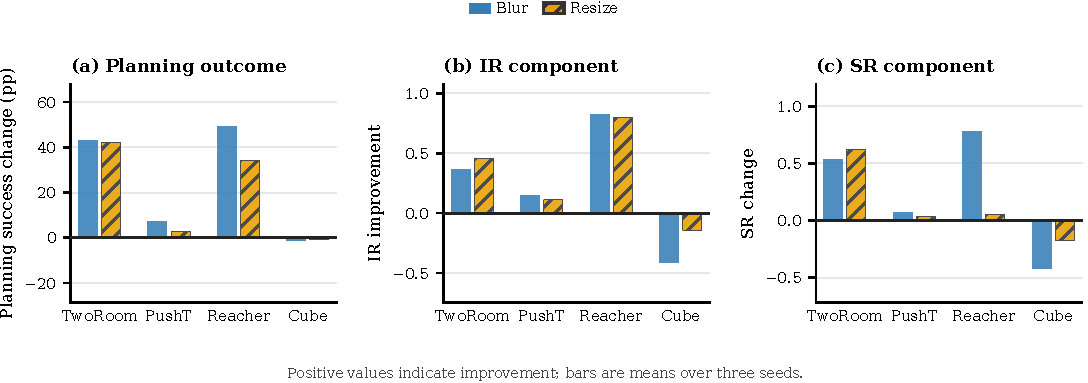
\includegraphics[width=\linewidth]{fig_cross_stressor_components_v1.pdf}
\caption{Changes from the unaugmented checkpoint to the checkpoint trained at $\stdmax{}=0.08$ under
blur and resize. Panels show (a) planning-success change in percentage points,
(b) IR improvement $1-\mathrm{IR}^{\mathrm{rel}}_q$, and (c) SR change. Bars
are means across three training runs, and positive
values indicate improvement.}
\label{fig:cross-stressor-components}
\end{figure}

\begin{table}[H]
\centering
\caption{Descriptive cross-stressor component summary. IR improvement is $1-\mathrm{IR}_{\rm rel}$ because the base value is 1; SR change is endpoint SR minus base SR. Spearman values correlate each component change with planning-success change. The leave-one-task-out (LOTO) range is obtained by omitting each task in turn and recomputing the pooled Spearman correlation. Binary agreement compares a positive component change with the prespecified positive behavior label. The final cell gives the 2.5th--97.5th percentiles from exact enumeration of all $4^4=256$ ordered task-cluster resamples, using linear interpolation. This is a sensitivity distribution, not a new-task population CI; the 24 paired rows are not IID.}
\label{tab:cross-stressor-components-v1}
\scriptsize
\setlength{\tabcolsep}{4pt}
\begin{tabular}{lrrrrl}
\toprule
Scope & $n$ & $\rho_{\rm IR}$ & $\rho_{\rm SR}$ & \shortstack{binary agreement\\IR / SR} & \shortstack{cluster-resampling\\sensitivity} \\
\midrule
Pooled & 24 & 0.854 & 0.913 & 0.917 / 0.917 & \shortstack{IR: [0.263, 0.950]\\SR: [0.352, 0.929]} \\
Blur & 12 & 0.874 & 0.953 & 0.917 / 0.917 & -- \\
Resize & 12 & 0.748 & 0.846 & 0.917 / 0.917 & -- \\
\midrule
TwoRoom & 6 & 0.543 & 0.543 & 1.000 / 1.000 & -- \\
PushT & 6 & 0.464 & 0.603 & 0.667 / 0.667 & -- \\
Reacher & 6 & 0.886 & 0.886 & 1.000 / 1.000 & -- \\
Cube & 6 & -0.086 & -0.543 & 1.000 / 1.000 & -- \\
\midrule
LOTO range & 18 & [0.720, 0.911] & [0.846, 0.901] & -- & -- \\
\bottomrule
\end{tabular}
\end{table}


\begin{table}[H]
\centering
\caption{Diagnostic ablation on 24 paired blur/resize endpoints. Each metric predicts improvement when its endpoint-to-reference ratio is below one; no threshold is fitted or transferred. Spearman correlation relates diagnostic improvement, defined as one minus this ratio, to planning-success change. Correct/24 and BA compare the predicted sign with the prespecified behavioral label. The LOTO range recomputes pooled Spearman after omitting each task; the 24 pairs are clustered within four tasks.}
\label{tab:cross-stressor-diagnostic-ablation}
\small
\setlength{\tabcolsep}{4pt}
\begin{tabular}{lcccc}
\toprule
Diagnostic & Spearman & Correct / 24 & BA & LOTO Spearman range \\
\midrule
Encoder only & 0.859 & 20 & 0.778 & [0.725, 0.901] \\
One-step rollout & 0.738 & 20 & 0.778 & [0.454, 0.877] \\
Zero actions & 0.805 & 21 & 0.833 & [0.626, 0.877] \\
Cross-anchor action shuffle & 0.780 & 21 & 0.833 & [0.586, 0.869] \\
Temporal action shuffle & 0.844 & 22 & 0.889 & [0.678, 0.923] \\
Recorded-action ACPC & 0.854 & 22 & 0.889 & [0.720, 0.911] \\
\bottomrule
\end{tabular}
\end{table}


\FloatBarrier
\section{Local Sensitivity under Gaussian Noise}
\label{sec:appendix-local-sensitivity}

To relate ACPC under Gaussian noise to local model sensitivity, consider a
small isotropic perturbation $\delta x\sim\mathcal N(0,\sigma^2 I)$. Let $J_E$
and $J_G$ be the Jacobians of the encoder and rollout map, evaluated along the
clean input. A first-order expansion gives
\[
\Delta G=J_GJ_E\,\delta x+o(\|\delta x\|_2).
\]
Writing $A=J_GJ_E$ and using
$\mathbb E[\delta x\delta x^\top]=\sigma^2I$, we obtain
\begin{equation}
\mathbb E\!\left[\|A\delta x\|_2^2\right]
=\operatorname{tr}\!\left(
A\,\mathbb E[\delta x\delta x^\top]A^\top
\right)
=\sigma^2\operatorname{tr}(AA^\top)
=\sigma^2\|A\|_F^2,
\label{eq:local-gaussian-sensitivity}
\end{equation}
Therefore, for small $\sigma$,
\[
\mathbb E[\|\Delta G\|_2^2]
\approx \sigma^2\|J_GJ_E\|_F^2.
\]
The squared Frobenius norm of the composed Jacobian thus measures how strongly
the encoder--rollout path locally amplifies Gaussian observation noise.
Jacobian Frobenius norms have previously been used to measure and regularize
local representation sensitivity~\citep{rifai2011contractive}. We estimate
\[
\|J_GJ_E\|_F^2
=\operatorname{tr}\!\left[(J_GJ_E)^\top(J_GJ_E)\right]
\]
with Rademacher probes and the Hutchinson
estimator~\citep{hutchinson1989stochastic}. Jacobian--vector products compute
these estimates without constructing the full Jacobian. In every task, both
the finite-difference and Jacobian-based estimates are lower for the
noise-augmented checkpoint (\Cref{fig:local-gaussian-sensitivity}). This result
is consistent with Gaussian-noise augmentation reducing ACPC by lowering the
local sensitivity of the encoder--rollout path. The analysis applies only near
the evaluated inputs and does not provide a global robustness guarantee.

\begin{figure}[t]
\centering
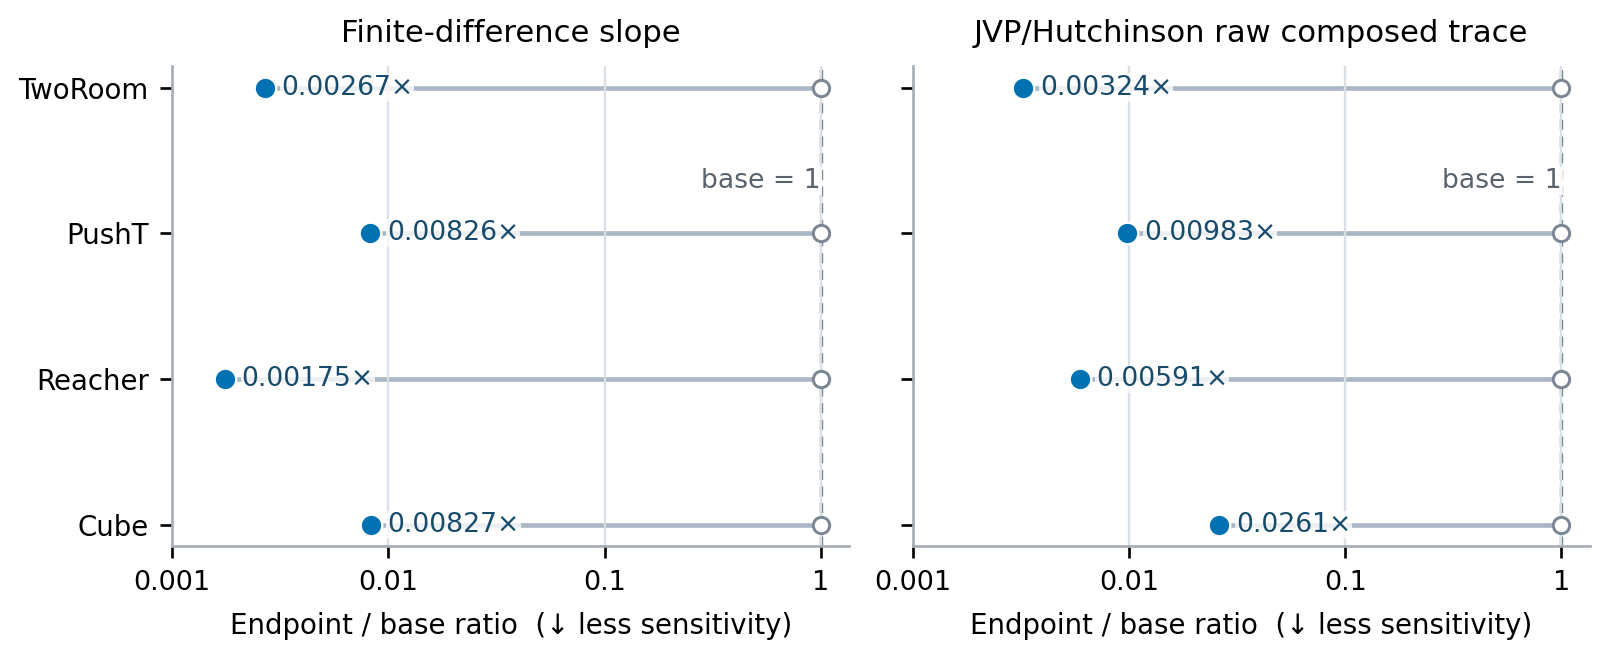
\includegraphics[width=0.88\linewidth]{fig_gaussian_sensitivity_main.png}
\caption{Ratio of local sensitivity for the Gaussian-noise-augmented
checkpoint to that of the unaugmented checkpoint. We report a
finite-difference estimate and a JVP-based Hutchinson estimate of the composed
Jacobian's squared Frobenius norm. Both estimates are below one for every task,
indicating lower local sensitivity after augmentation. These local
measurements do not establish task performance or global robustness.}
\label{fig:local-gaussian-sensitivity}
\end{figure}

\FloatBarrier
\section{Adaptive-CEM Selection Regret}
\label{sec:appendix-planner-protocol}

The selection-regret analysis does not use task-success labels. We evaluate
the unaugmented and $\stdmax{}=0.08$ checkpoints from every task and training
run. For each checkpoint, we use 100 histories and apply perturbations at
severities $0.02$, $0.05$, and $0.08$. Each clean or perturbed CEM run uses 64
candidate action sequences, eight elite candidates, eight iterations, and a
five-step prediction horizon. The paired runs start from the same proposal and
use the same random samples, but each run updates its proposal using its own
elite candidates.

The planner uses the squared distance between the predicted endpoint and the
goal embedding:
\[
C_j=\|x_j-g\|_2^2.
\]

For each CEM run, we compute ACPC for every candidate under that candidate's
action sequence. We summarize the candidate pool by the q90 ACPC at horizons
one and five. Let $\mathbf a$ be the plan selected from the clean history and
$\tilde{\mathbf a}$ the plan selected from its perturbed counterpart. The
regression target is the extra predicted cost of the perturbed-history plan
when both plans are evaluated from the clean history:
\[
\bigl[C_h(\tilde{\mathbf a})-C_h(\mathbf a)\bigr]_+.
\]

Within each training run, we fit ridge regressions on three tasks and evaluate
them on the remaining task, rotating through all four choices.
Each regression feature is standardized using the mean and standard deviation
computed from the three training tasks. The same values are used to standardize
features from the remaining test task. The target is
$\log(1+\text{selection regret})$, without further standardization. MAE is
computed on this scale and averaged equally across the four test tasks.
The relative MAE reduction is computed separately for each
training run before reporting the mean and sample standard deviation across
the three runs. This experiment evaluates whether ACPC reflects the model-cost
effect of a CEM selection change; it does not evaluate simulator return.

\Cref{tab:regression-target-scales} summarizes the target values predicted in
\Cref{sec:exp-target-aligned,sec:exp-planner}.
\begin{table}[H]
\centering
\caption{Summary statistics of the regression targets. The targets are
prediction-error change $d$ in \Cref{sec:exp-target-aligned} and
$\log(1+\text{selection regret})$ in \Cref{sec:exp-planner}.
Each task includes 288 and 1,800 samples, respectively, pooled across the
three training runs. SD denotes the standard deviation of target values,
not uncertainty in the mean.}
\label{tab:regression-target-scales}
\small
\begin{tabular}{lrrrr}
\toprule
& \multicolumn{2}{c}{Prediction-error change $d$}
& \multicolumn{2}{c}{$\log(1+\text{selection regret})$} \\
\cmidrule(lr){2-3}\cmidrule(lr){4-5}
Task & Mean & SD & Mean & SD \\
\midrule
TwoRoom & 8.756 & 6.518 & 2.123 & 2.188 \\
PushT & 6.725 & 5.653 & 2.170 & 2.077 \\
Reacher & 8.335 & 5.666 & 2.080 & 2.312 \\
Cube & 9.772 & 6.900 & 2.189 & 2.243 \\
\bottomrule
\end{tabular}
\end{table}

